\chapter{CNG Channels}
\label{chap:CNG_channel}

\section{CNG channels}
\label{sec:CNG_channel}

Cyclic nucleotide-gated  (CNG) ion channels or CNG channels are ion channels
that function in response to the binding of cyclic nucleotides (e.g. cGMP and cAMP)
and either a depolarization or a hyperpolarization event.
The CNG channels are significant in sensory transduction as well as cellular
development.
\url{http://en.wikipedia.org/wiki/Cyclic_nucleotide-gated_ion_channel}

A CNG channel consists of four subunits around a central pore. Each protein
subunit consists 6 transmembrane segments (S1-S6), a P-loop, intracellular amino
terminal region, and carboxy terminal region. The P-loop and S6 segments around
the pore, which plays a role in ion conduction. There is a cyclic nucleotide
binding domain (CNBD) and connection region to the S6 segment in the carboxy
terminal. There is a post-CNDB region in the amino terminal. CNG channels are
non-selective ion channels.

CNG channel homologs in Caenorhabditis elegans, Drosophila melanogaster, and
Limulus polyphemus have unknown functions. Studies have shown homologs in C.
elegans might have functions in chemosensation.

\begin{itemize}
  \item HCN current - Sect.\ref{sec:HCN-channels}
\end{itemize}
% \section{HCN channels (sinoatrial node in heart)}
% 
% 

\section{HCN channels (Ih or If - funny channels: mixed $\Na$ and $\K$)}
\label{sec:HCN-channels}
%\section{Funny channels }

HCN channels were first identified in 1976 in the heart by
Noma and Irisawa, and characterized by Brown and
Difrancesco and Weiss and his colleague. The general structure of HCN channels
resemble the structure of $\K$ channels with 4 subunits, each with 6TM/P
(Sect.\ref{sec:6TM/P}).
HCN channels are not present in some animals, such as the nematode {\it C.
elegans}.

HCN channels are non-selective cation channels, i.e. permeable to both $\Na$ and
$\K$ ions, with a $\Na$/$\K$ permeability ratio of about 1:5.
Each HCN channel has 4 either identical or non-identical subunits of
hyperpolarization-activated, cyclic nucleotide-gated (HCN) isoforms, encoded by
one of the four genes (Sect.\ref{sec:HCN-channel-structure}).


HCN channes are also classified as members of the voltage-gated $\K$ channels
(Sect.\ref{sec:Kv_channel}, as it has 6 TM domains (S1-6) with S4 is the
Voltage-sensor), and CNG channels (Sec.\ref{sec:CNG_channel}). The cyclic
nucleotide binding domain (CNBD) is in the C-terminus.


The channels are activated by hyperpolarization at voltages negative to $\sim $
-50 mV, and the typical reversal potential of HCN channel is -30
mV (higher than the normal threshold for generating AP in neuron) (Kase et al.,
2002).
The channels plays an important role in regulating neuronal excitability and
thus underline the rhythmic activities in the heart and brain.

They have given different names:
\begin{itemize}
  \item {\bf in the heart} (funny current): $I_f$ or $\IKf$ current, pacemaker
  channels.

  \item {\bf in the CNS}: HCN channels or $I_h$ (Sect.\ref{sec:Ih-current})
  
%  (other names: $I_h, I_q, I_f$ (funny currents)) 
\end{itemize}

\subsection{-- structure}
\label{sec:HCN-channel-structure}

An HCN channel as a tetramer, in which each subunit is encoded by one of the
four genes: : {\it HCN1, HCN2, HCN3}, or {\it HCN4}.
Ion channels encoded by each of the isoforms have differing biophysical
properties (such as speed of gating and sensitivity to cAMP), and are also
differentially distributed throughout the brain.


Once activated, they generate an excitatory inward current that can cause an
inhibition effect (5-10 mV depolarization effect) on EPSP. 
\begin{enumerate}
  \item HCN4 = slowly gating and strongly sensitive to cAMP
  \item HCN1 = more positive threshold for activation, fastest activation
  kinetics, yet lowest sensitive to cAMP
  \item HCN2 = intermediate properties
  \item HCN3 = intermediate properties
\end{enumerate}
Functionally, they differ from each other in terms of time constant of
activation with HCN1 the fastest, HCN4 the slowest and HCN2 and HCN3
intermediate.


The primary structure indicates six transmembrane segments, a positively charged
S4 segment, and the GYG pore sequence found in most known K+-selective channels
(Sect.\ref{sec:structure-K-channel}.
HCN channels also exhibit a highly similarity to CNG-gated channel
(Sect.\ref{sec:CNG_channel}) in the cyclic nucleotide-binding domain near the
COOH terminus.

\subsection{-- distribution}
\label{sec:HCN-channels-HCN1}

HCN1 and HCN2 are the main brain isoforms
\begin{itemize}
  \item HCN1 predominant in the neocortex and hippocampus, 
  

  \item HCN2 predominant in the thalamus.
  
  
  \item HCN3 has diffuse but low-level distribution in the brain, while 
  
  \item HCN4 is a subtype present mostly in thalamic relay neurons
\end{itemize}

\subsection{------ HCN1}	
\label{sec:HCN1-distribution-pyramidal-neuron}

There is an abundant expression of HCN1 in the layer 5 dendrites (Notomi and
Shigemoto, 2004; Santoro et al., 2004). However, it is not uniform; but vary
with distance from the soma.

Dendritic HCN1 channels normalize synaptic inputs in the cortical and
hippocampal neurons.  Current density of HCN channels increases along with the
distance from the soma in hippocampal and neocortical pyramidal neurons.

(Williams and Stuart, 2000; Berger et al., 2001) reported a significantly higher
density of Ih channel at distal dendritic sites. There are be 3 factors that
determine such differenc: i (single channel current), N (number of channels in
the region), and $P_o$ (the opening probability of channel). As there is no
evidence to supports the fact that Ih at distal sites has a higher opening
probability or higher single channel current, it is believed that the density
increases at distal sites. In deed, Ih channel number increases exponentially
with distance, i.e. Ih current density increases e-fold with every 325 $\mum$,
reaching densities as high as $\approx$ 550 channels/$\mum^2$ at distal dendritic sites
(Sect.\ref{sec:tufted-dendrite}). These high channel densities generate significant
membrane voltage noise (Kole et al., 2006).
\begin{itemize}
  \item about 40 Ih channels found in the somatic patch at site 120$\mum$
  from the soma.
  \item about 2500 Ih channels found in the dendritic patch at site 900$\mum$
  from the soma.
\end{itemize}
This suggests channel density 9-550 channels per $\mum^2$, given the estimate
membrane patch area is about 4.5$\mum^2$ (Engel, Jonas 2005).

HCN1 channel depolarized the soma by 10 to from -89 mV to -79 mV; and set the membrane
potential in the very distal tuft branches to  -65 mV.


\subsection{-- regulation factor}

All isoforms yield currents that are activated by hyperpolarization, carry K+
and Na+, are blocked by Cs+ in a voltage-dependent way, and are modulated by a
direct action of cAMP on the cytoplasmic side of the channel.

They, however, have different relative rates of activation and deactivation.
\begin{enumerate}
  \item HCN1: fastest kinetics to voltage change (i.e. tens of miliseconds),
  followed by HCN2 (several hundreds of miliseconds) and HCN4
  
  Half-maximal activation voltage (V1/2) is -73 mV (HCN1), -92 mV (HCN2), -81 mV
  (HCN4).
  
  The voltage dependence can be interpreted by assuming that Cs+ blocks after
  crossing ~66\% of the electrical field to reach its binding site.
  On the other hand, the concentration of Cs+ required to block
50\% of current was 15 mM for HCN2 channels, compared with 2.2 mM in Purkinje
fibers, implying that channels in this tissue are unlikely to be composed of
HCN2 subunits only
  
  \item efficacy of cAMP action has been found to
differ between isoforms: HCN1 being far less responsive than HCN2 and HCN4

HCN1 is virtual insensitivity to cAMP, i.e. very less membrane shift in
activation. Maximal shift of activation curve (whole-cell recording): 2-6.7 mV
(HCN1); 12-15 mV (HCN2); and 15.2-23 mV (HCN4)

Half-activation of [cAMP] is 0.5 $\muM$ for HCN2, closed to that of
0.2$\muM$ found in rabbit SAN.

  \item mHCN2 is 10x less sensitive to cGMP compared to cAMP
  
  This is similar to the relative sensitivity of If in the SAN to cGMP and cAMP

 \item a number of proteins are known to interact with HCN
subunits, such as Filamin A or TRIP8b
(Gravante et al., 2004; Santoro et al.,
2004).

\end{enumerate}

The current is activated by voltage (upon hyperpolarization) with a threshold of
($I_f$: -40 to -50 mV in SAN) and by intracellular signaling cascades, which
contain cyclic AMP (binding site near the C terminus of HCN), PIP2 (shift the
$V_m$-dependency through a different mechanism than cAMP), and TRIP8b.

It carries the inward current, which generates
the diastolic depolarization, eventually leading to the
threshold for Ca2+ channel activation and action potential firing


cAMP (cyclic adenosine monophosphate) binds directly to HCN channel and
increases the $P_o$. NOTE:
\textcolor{red}{Sympathetic stimulation raises cAMP level and shift the
activation range of HCN current to a more positive voltage and therefore
increase the max(dV/dt)}. Parasympathetic stimulation has the opposite effect, i.e.
decreasing the heart rate by increase $P_o$ of $\K$ channels but decrease $P_o$
of $\Ca$ channels.

\subsection{-- conductance}

The ratio $\Na$:$\K$ conductance ratio is 1:3 to 1:5, deriving from reversal
potential of HCN channel in the range -20mV to -30mV.
However, HCN channels primarily conduct Na+ current under physiological conditions, thus depolarizing neuronal
membrane potential.
Voltage-dependent activation of HCN channels is also anomalous compared to most
other channels: HCN channels are fractionally open at resting potential, and
their activation increases with hyperpolarization from rest rather than with
depolarization as is common with other channels.


The first single-channel recordings of If in dissociated cardiac cells indicated
a small unitary conductance of 0.98 pS (DiFrancesco, 1986).

A recent recording of Ih in acutely dissociated CA1 neurons using excised
patch-clamp reported a 10-fold larger single-channel conductance of 10 pS
(Simeone et al., 2005), i.e. giving a large single-channel current ($\sim$ 1
pA).
However, such larg single-channel currents were not observed in previous
cellattached studies of native Ih currents in CA1 pyramidal neurons (Magee,
1998).

For heterologously expressed HCN subunits, the single channel conductance
was reported differently, with values of the HCN2 unitary conductance ranging
from 2.5 pS (Johnson and Zagotta, 2005) to $\approx$ 35 pS (Michels et al.,
2005).

Using nonstationary fluctuation analysis (NSFA), Kole at al. (2006) found that
in cell-attached patches from the dendrites of cortical layer 5 pyramidal
neurons, average unitary conductance of 680$\pm$30 fS (i.e. 0.68 pS) and is
uniform single channel conductance along the somato-dendritic axis. So, its
current has a tiny, single-channel conductance.
This may suggest that excised patchclamp recordings used in the other
studies disturb the single-channel properties of Ih.

Channel permate to both Na and K: Values of P$_\Na$/P$_\K$ ratio ranging from
0.25 to 0.41 have been reported for the cloned channels.

Given the wide spectrum of observed unitary conductances for voltage-dependent
channels (from 1 to 300 pS) (Hille, 2001), why If single-channel current is too
small?



\subsection{Ih current}
\label{sec:Ih-current}

{\bf in the CNS}: HCN channels or $I_h$ (Sect.\ref{sec:HCN-channels}). $I_h$
current controls and contribute to rhythmic firing, synaptic plasticity, etc.

Activated HCN channels are involved in the detection of coincidental synaptic
inputs. Because HCN channel conductance shortens the rise time and decay time of
the EPSPs through the decrease in membrane resistance.
This suppression filters out low-frequency inputs, and thus improves the
selectivity for synchronous synaptic inputs

\subsection{-- gating (agonist, antagonist)}

Ih currents evoked by hyperpolarizing pulses from a holding potential 25 mV
depolarized to the resting membrane potential. These currents could be blocked
by 82$\pm$7\% by bath application of 50 $\mu$M of the Ih antagonist ZD 7288
(BoSmith et al., 1993; Robinson and Siegelbaum, 2003), indicating adequate
specificity for Ih.

\subsection{If current}
\label{sec:funny-channel}
\label{sec:If-current}

{\bf in the heart}: $I_f$ or $\IKf$ current, pacemaker channels.
The molecular basis of $I_f$ current belongs to the {\bf
hyperpolarization-activated cyclic nucleotide-gated channels family (HCN)}
(Sect.\ref{sec:HCN-channels}).
HCN1 is expressed in cardiac sinoatrial but not atrial or atrioventricular
cells.
\begin{itemize}
  \item HCN4 was originally cloned from the SAN 

murine SAN has been shown to contain HCN1, HCN2, and especially HCN4

  \item HCN2 mRNA has been found in the mouse ventricle
  
  \item 
\end{itemize} 

The significance of this is that as the heart resets, or hyperpolarizes, after
each beat, If channels open, allowing positive ions to rush into the cell (the
so-called funny current), triggering another depolarization event and subsequent
cardiac contraction. This gives the heart its automaticity.

The subunits of $I_f$ in sino-atrial nodes have HCN4 as the main isoform, with
low levels of HCN1 and HCN2 \citep{Herrmann2011, Baruscotti2010, Brioschi2009}.
A similar current like $I_f$ in the central nervous system (CNS) is
called $I_h$ (Sect.\ref{sec:Ih-current}). 
  

\begin{mdframed}

The funny current (funny channel $I_f$) was first described in 1976 
in excitation/conducting cells (SA node, AV node, and Purkinje fibers of
conducting tissues) by Noma and Irisawa. This current is a mixed $\Na$-$\K$
current. The small $\Na$ leaky inward flux via $I_f$ channel allows the $\Na$ ions to constantly pour
into the cell, slowly depolarizing the membrane. The funny channel is not
voltage-gated but operates at voltage in diastolic range (from -60/-70 mV to
-40mV) to supply an inward current, and are thus continuously open when the
cell is at rest. The inherent leakiness of SA node fibers to $\Na$ ions is what
causes their self-excitation. Thus, $I_f$ channel is the common target of
drugs to control heart rate.

\end{mdframed}


Genetic alterations in $I_f$ channels can cause different cadiovascular
diseases: 
\begin{enumerate}
  \item inherited sinus bradycardia: S672R (a highly conserved residue in the
  CNBD of the HCN4)
\end{enumerate}


\url{https://en.wikipedia.org/wiki/Cyclic_nucleotide-gated_ion_channel}


\subsection{-- gating}

The kinetic features of native f-channel activation/deactivation cannot be
described satisfactorily by the use of Hodgkin-Huxley (HH) description
(DiFrancesco 1984).  To account for these features, a complex kinetic model
based on the coexistence of a "delaying" and a proper "gating" process and
involving five voltage-dependent gating variables of three different types had
been previously proposed (DiFrancesco 1984). 

If is activated by hyperpolarization at -40mV to -50mV in SAN of rabbit,
Fig.\ref{fig:If_SAN}. 
\begin{itemize}
  
  \item  ISO: $\beta$-Adrenergic agonists increase If at diastolic potentials by
  shifting the activation curve to more positive voltages.
  
MECHANISM:  cAMP-induced shift ranges from 11 to 14 mV in the SAN, accounting
for most of the additive shift of about 18 mV produced by maximal stimulation
with $\beta$-adrenergic and muscarinic agonists.
A half-maximal shift is obtained with a cAMP concentration of 0.2 $\muM$
(Sect.\ref{sec:cAMP-dependent_pathway}).

  \item ACh: Muscarinic agonists have opposite effects on
If and shift the activation curve to more negative voltages, i.e. less inward
current is available at diastolic potentials, causing a decreased slope of this
phase and decelerating heart rate.

  \item Pronase: application of
pronase to excised patches from SAN myocytes shifts the activation curve of If
to more depolarized potentials by about 57 mV without affecting the fully
activated relation

HERE: the effects of cAMP on the current are completely abolished

\end{itemize}
The fully activated current/voltage relation
reverses near -10/-20 mV in physiological solutions as a consequence
of the channel mixed permeability to Na+ and K+, a
second unusual property of If. 

\begin{figure}[hbt]
 \centerline{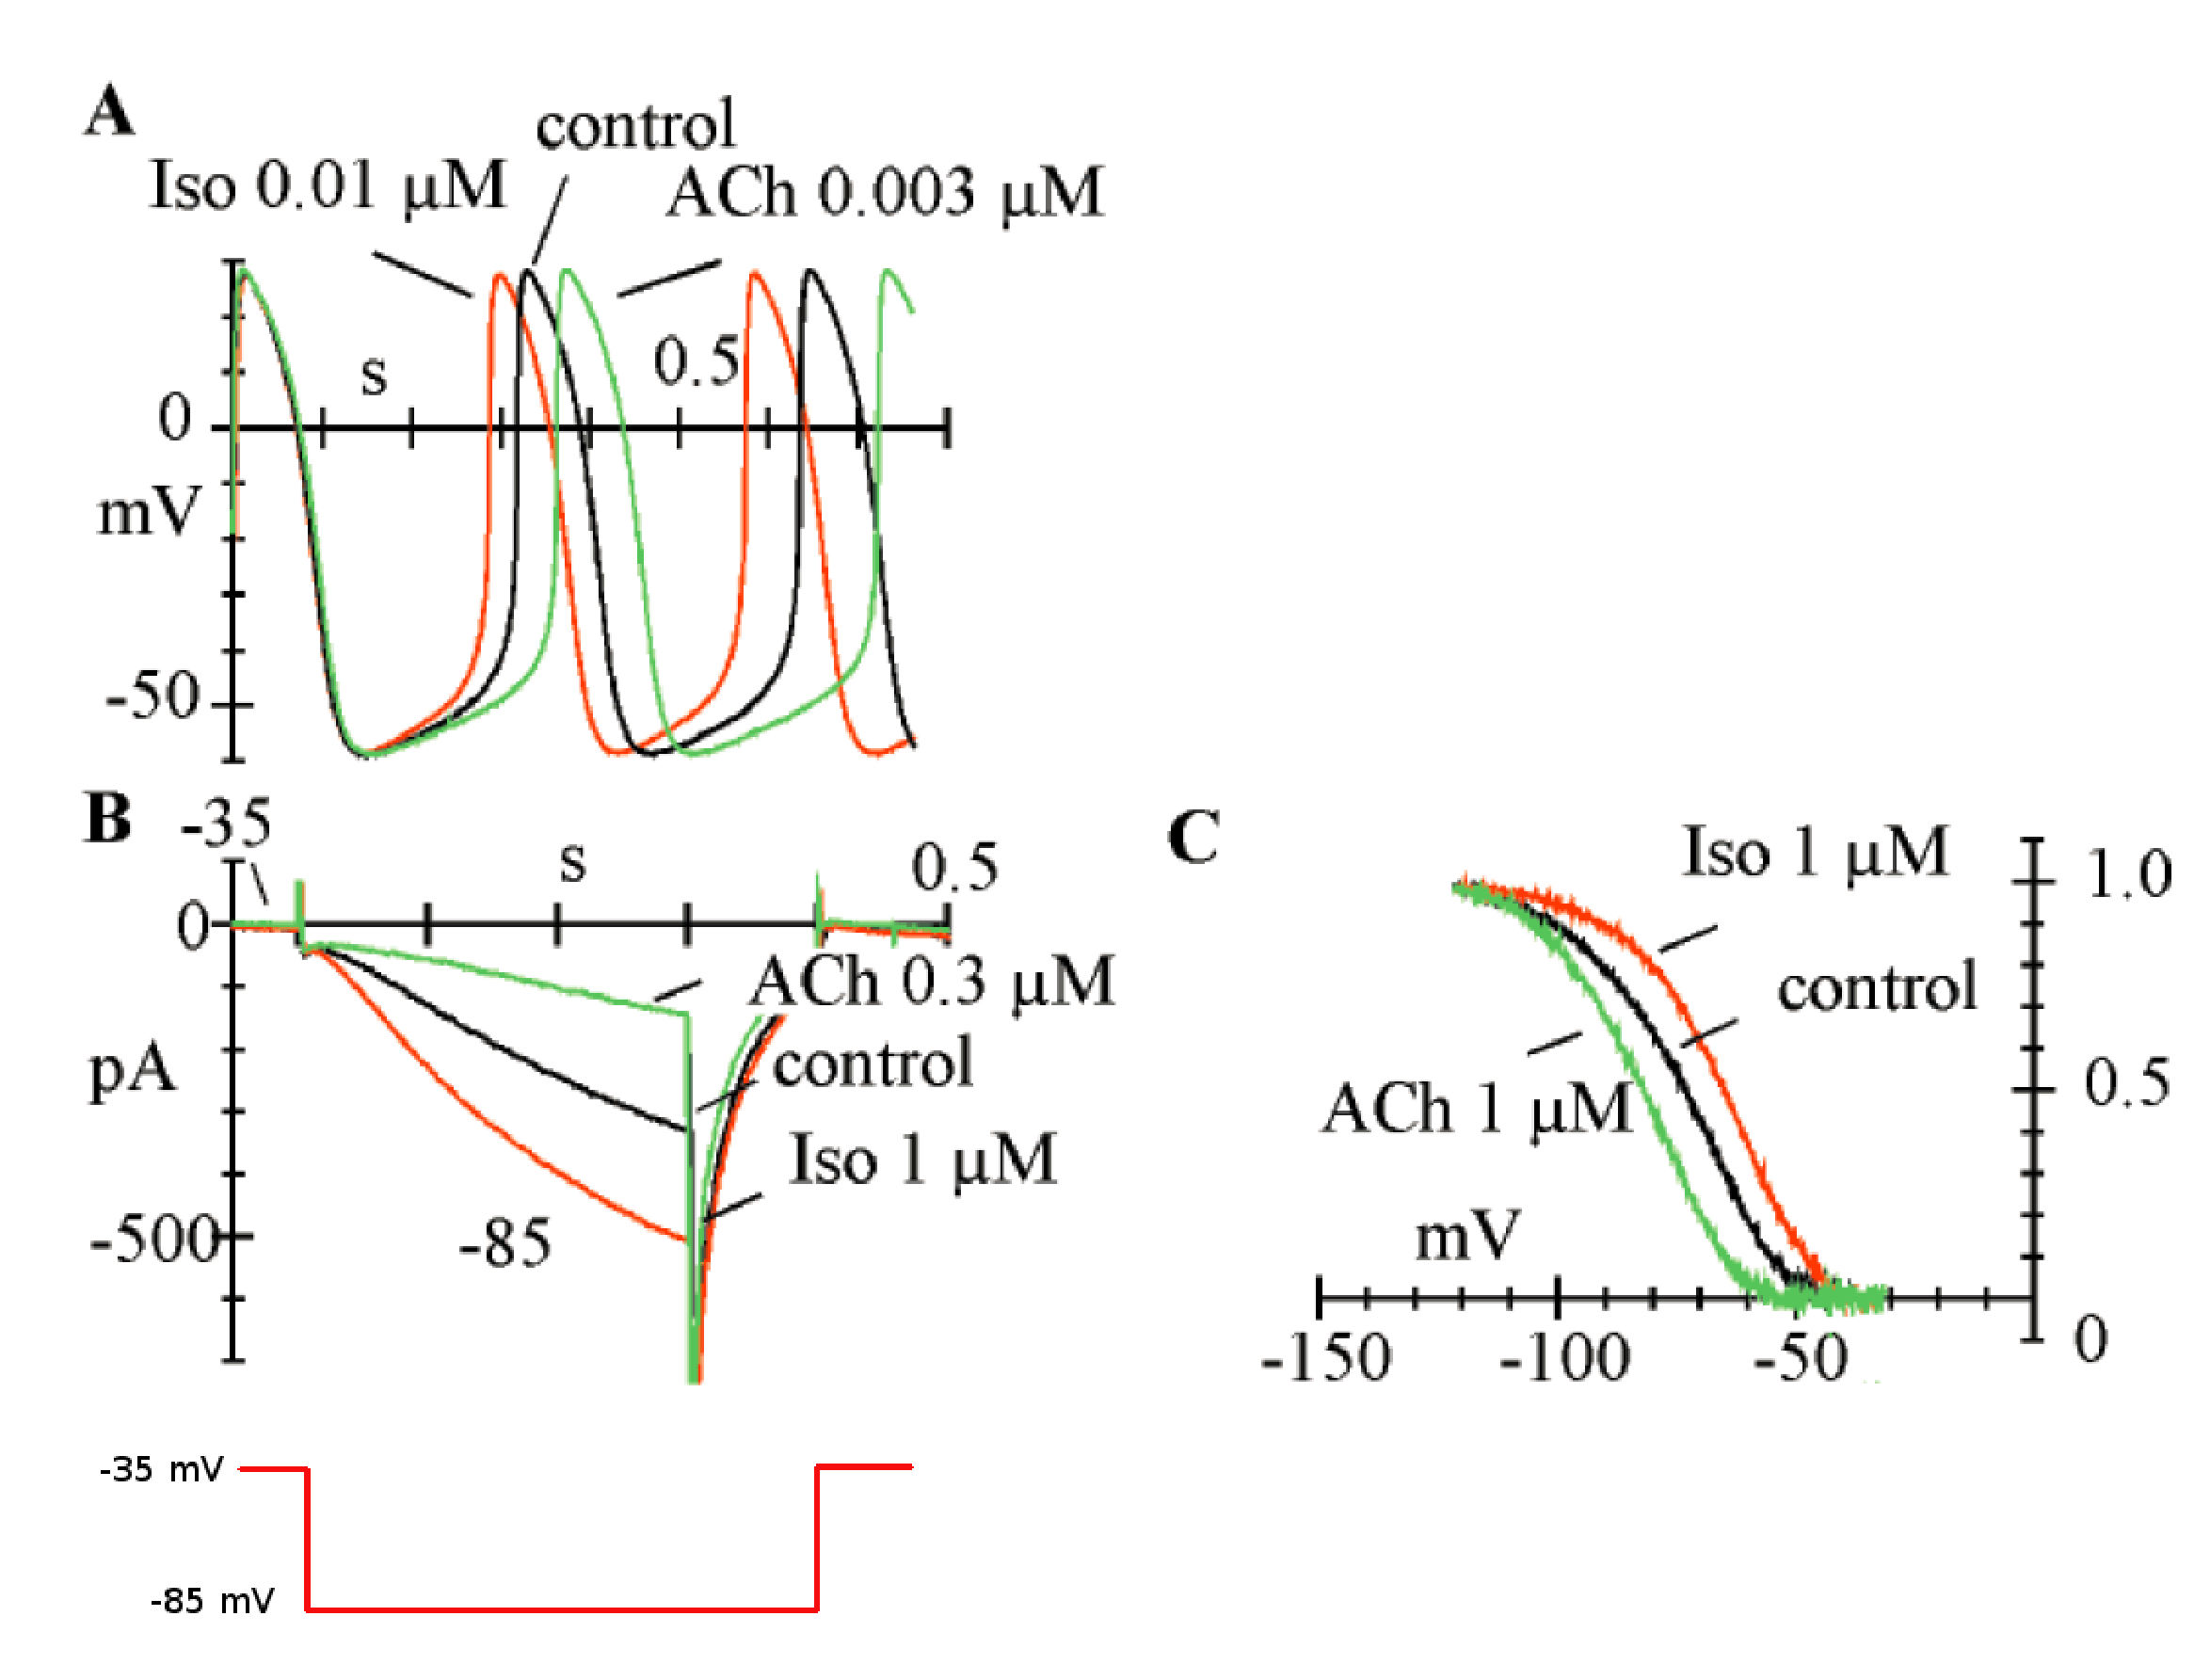
\includegraphics[height=7cm]{./images/If_SAN.eps}}
\caption{If current in SAN (cardiac sinoatrial node) of rabbit. (A) Ctrl, ISO
and ACh effect. The change in the frequency (i.e. increase by ISO, and slower by
ACh) due to its effect on the rate of diastolic depolarizaiton. (B) Upon a
hyperpolarizing step to -85 mV from -35 mV, If current is elicited . ISO makes
the If current more sensitive to Vm, i.e. providing more inward current at
diastolic potentials. (C) However, both ACh and ISO do not shift the peak of If,
which means they do not affect the fully activated current}
\label{fig:If_SAN}
\end{figure}

It is suggested that an inhibitory mechanism of If current located at the COOH
terminus. This inhibitory mechanism is
\begin{itemize}
  \item partially removed upon cAMP binding
  
  \item completely removed upon pronase-induced cleavage of the COOH terminus.
\end{itemize}
This leads to the hypothesis that the
COOH terminus of If channels contributes to gating by inhibiting
channel opening and that the shifting action of cAMP is
due to attenuation of the inhibitory process. \citep{accili2002} (Accili et
al., 2002)

The allosteric hypothesis: This model suggests that voltage and
cAMP use a common mechanism to increase the channel
open probability. According to the allosteric model, channel
opening is the combination of two processes
\begin{itemize}
  \item displacement of Voltage sensor (one for each of 4 subunits) from
  reluctant to willing state
  
  
  \item allosteric closed-to-open transitions involved concerted arrangement of
  all 4 subunits
\end{itemize}
The probability of channel opening increases every time one voltage sensor
switches to the "willing" state.

